\section{Methodology}
\label{sec:methodology}

\subsection{Previous Attempts} %Tried methods
At first, we tried to rely solely on descriptors. The first proposed method was a combination of local and global descriptors that describe various features on the images. We used the SIFT, ORB and SURF descriptors that are local descriptors. Then, using global descriptors we tried to tie the identified segments together. These alone however were not sufficient. This method was unable to capture a more significant connection between the separate images and therefore was not able to be used to reconstruct the room itself. An underlying problem of this method was that local and global descriptors capture different types of information, which are not easily associated with one another.

A different method tried was the involvement of a machine learning model with a well-trained CNN. We hoped that there were some hidden connection points that are accurately detectable using a neural network. This produced some results, however the use of this model was limited only to a set of cases. In these cases the image sets exceeded the minimal amount of images needed to map out a room with no blindspots. Most image sets consisted of images that had many repeating regions in them, which in our study is a redundant set. We aim to process and reconstruct a room with as few images as possible and minimal amount of repeating image regions.   

A purely algorithmic approach was also tried. There were some promising results using graphs and edge detection. Using this method, we detected the edges of all walls with a modified version of Harris-Corner detection. Then, the developed algorithm managed to connect all corners of a non-cuboid shaped room using graph theory. This ended up not fitting our study, since detecting only the edges of a room is not enough to fully detail it. Therefore, the full recostruction of a room was determined to be impossible using this method. This method took some inspiration from \cite{9707088}, as this paper also used a similar method to determine edges of a room.


\subsection{Detection of distinct segments} %Segment detection
For segment detection, we revisited local descriptors. Using these descriptors we were able to detect spots in the image that can be described by some feature. These spots are called segments. For example color or shape of a given object can be detailed using these descriptors. Using different types of local descriptors, the algorithm looks for the following features in an image: color, shape, texture, orientation and boundaries of a segment. Some different extractable characteristics are presented in Figure \ref{fig:desc_data}.

\begin{figure}[htbp]
    \centering
    \begin{subfigure}[b]{0.38\textwidth}
        \centering
        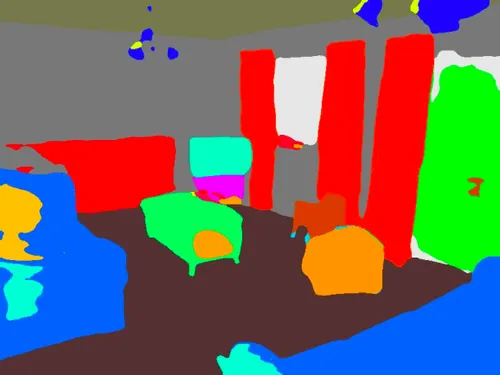
\includegraphics[width=\textwidth]{images/objdet.png}
        \caption{Detecting objects using descriptors}
        \label{fig:desc_objdet}
    \end{subfigure}
    \hfill
    \begin{subfigure}[b]{0.38\textwidth}
        \centering
        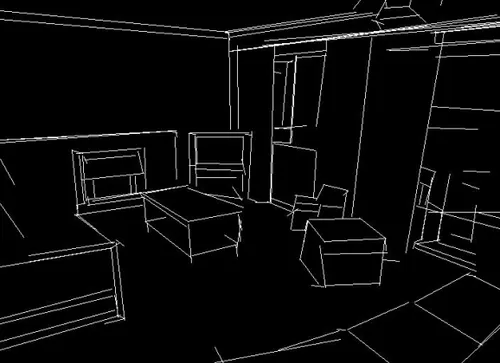
\includegraphics[width=\textwidth]{images/edgedet.png}
        \caption{Identifying edges using descriptors}
        \label{fig:desc_edge}
    \end{subfigure}
    \caption{Data processing using descriptors}
    \label{fig:desc_data}
\end{figure}

Some regions will only be detected once by one specific descriptor. However since we use multiple type of descriptors, more than one descriptor can find the same segment. This would be a problem, however the algorithm uses this to its advantage. It uses the redundant information to determine the easily detectable segments. For the sake of simplicity, in this paper a descriptor detailing a segment is called a representation.

After every possible detail is extracted from an image, we run these representations of segments through a filter that is able to separate the segments into a distinct set. An element of the set consists of a segment and its associated representations. The process of organizing the representations into this set happens by measuring the similarity of two representations against a threshold. If that threshold is reached, the similarity is deemed to be too great and therefore only one of the representation of the segment can remain as the main representation (it is proposed that a high chance of similarity means that the two representations detail the same segment). The unused segment representations are also saved in the set, but only one main representation can be the appointed segment of the set.

The process of this filtering is detailed in Algorithm \ref{alg:distinct}, which gives a rough outline of the control and data flow of the algorithm. The complexity of the algorithm is $O(n^2)$ where $n$ is the number of representations.
%algorithm to detail this set creation
\begin{algorithm}[H]
\caption{Building of the Segments Set}\label{alg:distinct}
\begin{algorithmic}
    \State \texttt{Declare set S}
    \State \texttt{Given representations in R}
    \For{ \texttt{representation r in R}}
        \State \texttt{Declare flag F for similarity}
        \For{\texttt{segment s in S}}
            \If{\texttt{r and s similarity > threshold}}
                \State \texttt{Add r as a representation to s}
                \State \texttt{Set F}
                \State \texttt{Raise confidence level of segment s}
            \EndIf
        \EndFor
        \If{F not set}
            \State \texttt{Add r as a segment to s}
            \State \texttt{Initialize confidence level of segment r}
        \EndIf
    \EndFor
\end{algorithmic}
\end{algorithm}


This filtering process also assigns a number to each segment in the set. This number is a so called confidence level, that is able to measure how confident the algorithm is in that this segment is a real, easily distinguishable one. A segment's confidence level is increased if a similar segment was found with a different descriptor. In this case, the algorithm assumes that now more than one descriptor found the same segment and therefore it is more likely that this segment is a real one. 

At the end of this process, we are left with a set of distinct segments, represented by different type of descriptors. Because of the heavy use of different types of feature detection and description, we maximize the number of detectable segments in an image set. The next stage of the process is the association of these segments.

\subsection{Association of Segments} %Segment Association
\label{subsec:assoc_segm}

The first task in the association of segments is determining the interesting and important key points. During the detection phase, some information is already saved about the individual representations, which decriptor found it, how high its activation level was and additional information based on the type of descriptor. While merging them into segments, these characterestics are inherited. Segments also have their confidence score. Based on all these factors, an interest score is calculated for each segment. Then the most important segments will be selected as the first key points.

In the following step, each key point gathers the similar segments around themselves. These groups are also called knots in this paper. An association likeliness score is calculated between each key point and each segment. This includes the similarity of characterestics of the two segments and their disctance. The factors that contributed heavily to the interest score of the key points are weighted more heavily here. Every segment with an association score above a certain threshold is associated with the given key point, it is placed inside its knot. Each segment can be part of multiple knots independently and there is no upper bound for the possible number of association. Therefore, this part of the process can be heavily parallelized to improve the algorithms performance.

These two steps are repreated iteratively. In the following iterations, the number of associations and their strength are also calculated into the interest score of the segments. This ensures that the different segments with different characterestics are selected in each iteration. The desired number of key points and the association threshold are both increased between iterations. While this approach ensures that more and smaller group of segments are gathered around the key points in each iteration, there is no direct hiearchy between them, since the new key points gather segments independently from their previous groups. The iteration of the association ends when a certain number of key points are selected.

This algorithm is summarized in Algorithm~\ref{alg:assoc}. The complexity of the algorithm is $O(nk)$ where $n$ is the number of segments and $k$ is the desired number of knots.

\begin{algorithm}[H]
\caption{Building of the Knots}\label{alg:assoc}
\begin{algorithmic}
\State \texttt{Declare set K}
\State \texttt{Given segments in S}
\State \texttt{Given desired number of key points as D}
\State \texttt{Given starting association threshold as T}
\State \texttt{Given starting desired number of key points as R}
\While{\texttt{Lenght of K < D}}
    \State \texttt{Declare set P}
    \For{\texttt{segment s in S}}
        \State \texttt{calculate interest score of s}
    \EndFor
    \State \texttt{select R segments from S with the highest interest score into P}
    \For{\texttt{key point k in P}}
        \For{\texttt{segment s in S}}
            \State \texttt{calculate association score a}
            \If{\texttt{a > T}}
                \State {\texttt{associate k and s}}
            \EndIf
        \EndFor
        \State \texttt{add k to K}
    \EndFor
    \State \texttt{increase T}
    \State \texttt{increase R}
\EndWhile
\end{algorithmic}
\end{algorithm}

Some examples of the final knots can be seen in Figure \ref{fig:knots_examples}. The colored parts represent the detected objects and the white lines represent the detected edges associated with the knot.

\begin{figure}[htbp]
    \centering
    \begin{subfigure}[b]{0.38\textwidth}
        \centering
        
\includegraphics[width=\textwidth]{images/knot1.png}
        \caption{Example identifying the curtains}
        \label{fig:knots_example_1}
    \end{subfigure}
    \hfill
    \begin{subfigure}[b]{0.38\textwidth}
        \centering
        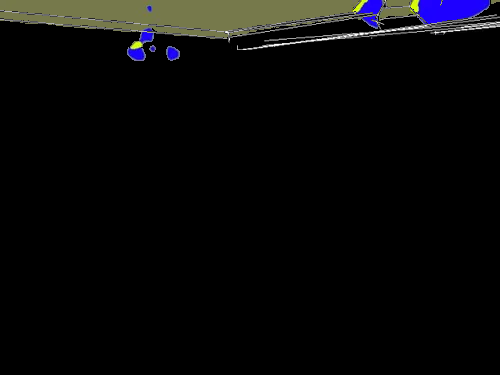
\includegraphics[width=\textwidth]{images/knot2.png}
        \caption{Example identifying the ceiling}
        \label{fig:knots_example_2}
    \end{subfigure}
    \caption{Examples of Possible Knots}
    \label{fig:knots_examples}
\end{figure}

\subsection{Connection of Knots} %Knots Connection
\label{subsec:connect_knots}

The next important step is creating a common depiction for each knot. These depictions are also called super segments. To create a super segment, the statistical data for the segments in the knot is calculated. This includes the number of segments and representations in the knot and individual statistics for each characteristic of the segments. For each value the mean, the median, the mode, the quartiles and the deviation are calculated.

Based on these statistics the connection strength score matrix, abbreviated to CSSM, is calculated. The matrix represents the connection strength of every super segment with every other super segment. To get the values for one of the super segments, first the difference between its statistics and every other super segment's is calulated, separately for each characteristic. The differences are ranked and based on the closest value each following one's score is increased. The strength scores are normalized, so for each the closest super segment's score will be one.

A simplified version of the algorithm, without detailing the per characteristics calculations, is shown in Algorithm~\ref{alg:buildcssm}. The complexity of the algorithm is $O(n^2)$ where $n$ is the number of knots.

\begin{algorithm}[H]
\caption{Building of CSSM}\label{alg:buildcssm}
\begin{algorithmic}
\State \texttt{Given super segments in S}
\State \texttt{N := length of S}
\State \texttt{Declare NxN matrix M }
\For{\texttt{i <- 1 to N}}
    \For{\texttt{j <- 1 to N}}
        \If{\texttt{i =/= j}}
            \State {\texttt{calculate connection strength score in M[i,j]}}
        \EndIf
    \EndFor
    \State \texttt{select m where M[i,m] is maximal}
    \For{\texttt{j <- 1 to N}}
        \If{\texttt{i =/= j}}
            \State {\texttt{M[i,j] := M[i,j] / M[i,m]}}
        \EndIf
    \EndFor
\EndFor
\end{algorithmic}
\end{algorithm}

A possible CSSM for four knots is shown in \autoref{table:example_cssm}. In this example, Knot A finds that Knot B has the closest connection with it, followed by Knot D and Knot C. It is worth noting that matrix is not necessarily symmetrical. Here Knot B estimates that its strongest connection is with Knot C, instead of Knot A.

\begin{table}[H]
    \centering
    \begin{tabular}{|c | c | c | c | c |}
        \hline
        \multicolumn{5}{|c|}{Connection Strenght Scores} \\
        \hline
        \diagbox{Source}{Target} & Knot A & Knot B & Knot C & Knot D \\
        \hline
        Knot A &  -  & 1.0 & 0.2 & 0.3 \\
        \hline
        Knot B & 0.8 &  -  & 1.0 & 0.1 \\
        \hline
        Knot C & 0.2 & 0.7 &  -  & 1.0 \\
        \hline
        Knot D & 0.1 & 0.3 & 1.0 &  - \\
        \hline
    \end{tabular}
    \caption{Example CSSM}
    \label{table:example_cssm}
\end{table}

\subsection{Defining a layout guess} % Process of recontruction

Taking the aforementioned depictions in the CSSM we attempt to create multiple graph structures that are separate from each other. For a given graph we take the nodes as the depictions. The edges for a given graph differ from graph to graph. These edges are weighted and  determined by a proximity value. If two given depictions' strength scores (calculated by the CSSM) are above the proximity value, an edge is formed between the associated nodes. Different graphs work with different proximity values and the strength scores differ from as well. For each graph a proximity value is selected and strength scores are calculated from a CSSM detailed in \ref{subsec:assoc_segm}. This CSSM takes into account different characteristics for each graph. More concretely, every time a different subsection of characteristics are used to define a CSSM. 

The proximity values are selected from a range. This range is defined by taking the CSSM strength scores and setting the range's limits to the first and third quartiles of the strength scores. Proximity values are then picked from this range to be used for the creation of different graphs. The process of defining graphs is detailed in Algorithm \ref{alg:graph}. The complexity of the algorithm is $O(n^2)$ where $n$ is the number of depictions.

\begin{algorithm}[H]
\caption{Defining the graphs}\label{alg:graph}
\begin{algorithmic}
\State \texttt{Given depictions in D}
\State \texttt{Given proximity range P}
\State \texttt{Given desired amount of graphs k}
\State \texttt{Define graph G with every depiction from D}
\For{\texttt{k}}
    \State \texttt{Define p proximity value from P}
    \State \texttt{Define CSSM strength scores in matrix C}
    \For{\texttt{depiction d1 in D}}
        \For{\texttt{depiction d2 in D}}
            \If{strength of d1 d2 > p}
                \State \texttt{Create edge between d1 and d2}
            \EndIf
        \EndFor
    \EndFor
\EndFor

\end{algorithmic}
\end{algorithm}

As a result of selecting distinct proximity values, we are left with graphs that have various combinations of edges defined. All graphs contain all depictions but the connections of depictioncs is different. The weight of the edges are the strength scores from CSSM. These graphs each define a layout and a relation between depictions, which in turn means it defines a structured layout between grouped segments. These layouts all function as guesses for the true layout, each guess having worked with different proximity value could have a different guess for the layout. Possible outputs resulting in this step can be seen in Figure \ref{fig:layoutguesses}.

\begin{figure}[htbp]
    \centering
    \begin{subfigure}[b]{0.38\textwidth}
        \centering
        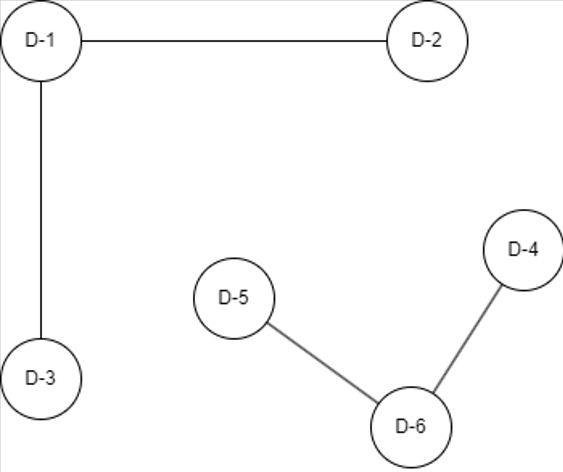
\includegraphics[width=\textwidth]{images/layoutguess1.png}
    \end{subfigure}
    \hfill
    \begin{subfigure}[b]{0.38\textwidth}
        \centering
        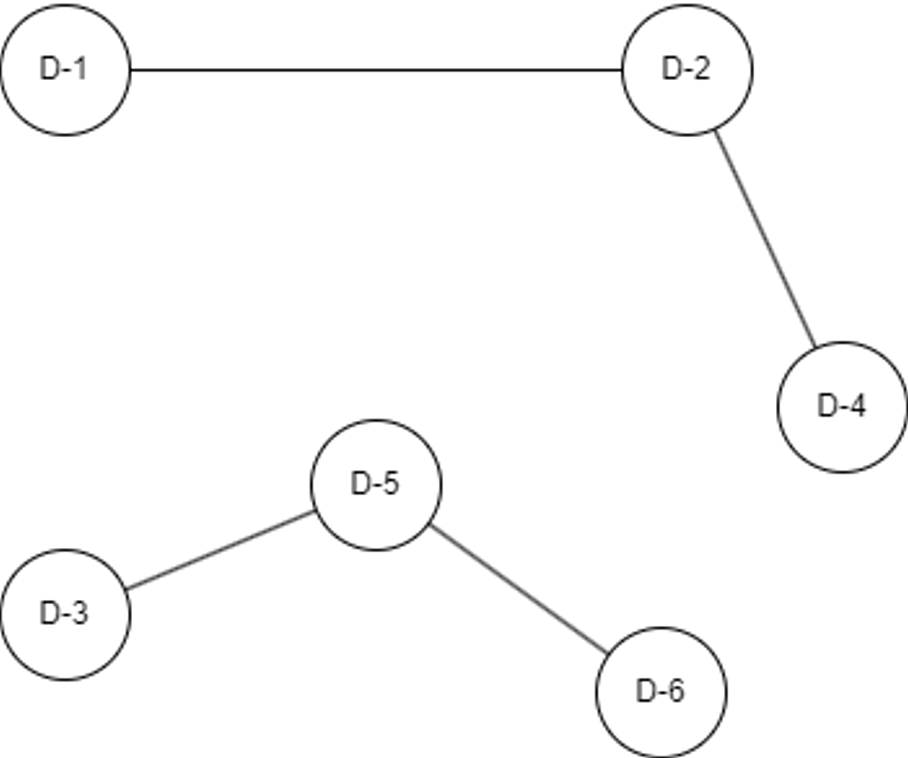
\includegraphics[width=\textwidth]{images/layoutguess2.png}
    \end{subfigure}
    \caption{Two possible layout guesses}
    \label{fig:layoutguesses}
\end{figure}

These graphs are then ran through an algorithm that detects the most commonly guessed edges (and therefore connections). Edges between depictions that are rarely defined are not taken into account. By having different CSSMs for each graph we give a chance for underrepresented edges to also make into the final layout guess. This method of selection produces one final layout that contains the most likely edges.


\subsection{Reconstructing a floor map}

Based on the final layout guess, a floor map can be reconstructed. To achieve this we take the depictions and using the edge characteristics (note that this edge characteristic is given by a descriptor, this is not the graph's edge), we map out an outline of the room. Since the graph's nodes are connected in the appropriate form, we can use the location and edge characteristics to accurately map out a room's walls and corners. Using the locations of the depictions, we could estimate the dimensions of the room. The final representation of a room consists of definition of two-dimensional points. The corners are represented by points in a cartesian coordinate system, for the sake of simplicity. Coordinates are represented in measures of centimeters. Since doors and windows also have distinct, detectable characteristics, these also get processed as depictions. Using the dimensional data provided by the graph these elements can also be properly placed in a fllor map. For the sake of uniformity, these are also represented as points with a special flag in their data, signaling that these points represent doors and windows.



